\documentclass[
    xcolor={svgnames,dvipsnames},
    hyperref={colorlinks, citecolor=DeepPink4, linkcolor=DarkRed, urlcolor=DarkBlue}
    ]{beamer}  % for hardcopy add 'trans'


\mode<presentation>
{
  \usetheme{Pittsburgh}
  % or ...
  \setbeamercovered{transparent}
  % or whatever (possibly just delete it)
}

\usefonttheme{professionalfonts}
%\usepackage[english]{babel}
% or whatever
%\usepackage[latin1]{inputenc}
% or whatever
%\usepackage{times}
%\usepackage[T1]{fontenc}
% Or whatever. Note that the encoding and the font should match. If T1
% does not look nice, try deleting the line with the fontenc.

%\usepackage{fontspec}
%\setmonofont{CMU Typewriter Text}
%\setmonofont{Consolas}

%%%%%%%%%%%%%%%%%%%%%% start my preamble %%%%%%%%%%%%%%%%%%%%%%

\addtobeamertemplate{navigation symbols}{}{%
    \usebeamerfont{footline}%
    \usebeamercolor[fg]{footline}%
    \hspace{1em}%
    \insertframenumber/\inserttotalframenumber
}


\usepackage{graphicx}
\usepackage{amsmath, amssymb, amsthm}
\usepackage{bbm}
\usepackage{mathrsfs}
\usepackage{xcolor}
\usepackage{fancyvrb}

% Quotes at start of chapters / sections
\usepackage{epigraph}  
%\renewcommand{\epigraphflush}{flushleft}
%\renewcommand{\sourceflush}{flushleft}
\renewcommand{\epigraphwidth}{6in}

%% Fonts

%\usepackage[T1]{fontenc}
\usepackage{mathpazo}
%\usepackage{fontspec}
%\defaultfontfeatures{Ligatures=TeX}
%\setsansfont[Scale=MatchLowercase]{DejaVu Sans}
%\setmonofont[Scale=MatchLowercase]{DejaVu Sans Mono}
%\setmathfont{Asana Math}
%\setmainfont{Optima}
%\setmathrm{Optima}
%\setboldmathrm[BoedFont={Optima ExtraBlack}]{Optima Bold}

% Some colors

\definecolor{aquamarine}{RGB}{69,139,116}
\definecolor{midnightblue}{RGB}{25,25,112}
\definecolor{darkslategrey}{RGB}{47,79,79}
\definecolor{darkorange4}{RGB}{139,90,0}
\definecolor{dogerblue}{RGB}{24,116,205}
\definecolor{blue2}{RGB}{0,0,238}
\definecolor{bg}{rgb}{0.95,0.95,0.95}
\definecolor{DarkOrange1}{RGB}{255,127,0}
\definecolor{ForestGreen}{RGB}{34,139,34}
\definecolor{DarkRed}{RGB}{139, 0, 0}
\definecolor{DarkBlue}{RGB}{0, 0, 139}
\definecolor{Blue}{RGB}{0, 0, 255}
\definecolor{Brown}{RGB}{165,42,42}


\setlength{\parskip}{1.5ex plus0.5ex minus0.5ex}

%\renewcommand{\baselinestretch}{1.05}
%\setlength{\parskip}{1.5ex plus0.5ex minus0.5ex}
%\setlength{\parindent}{0pt}

% Typesetting code
\definecolor{bg}{rgb}{0.95,0.95,0.95}
\usepackage{minted}
\setminted{mathescape, frame=lines, framesep=3mm}
\usemintedstyle{friendly}
%\newminted{python}{}
%\newminted{c}{mathescape,frame=lines,framesep=4mm,bgcolor=bg}
%\newminted{java}{mathescape,frame=lines,framesep=4mm,bgcolor=bg}
%\newminted{julia}{mathescape,frame=lines,framesep=4mm,bgcolor=bg}
%\newminted{ipython}{mathescape,frame=lines,framesep=4mm,bgcolor=bg}

% Typesetting code
\definecolor{bg}{rgb}{0.95,0.95,0.95}
\usepackage{minted}
\usemintedstyle{friendly}
\newminted{python}{mathescape,frame=lines,framesep=4mm,bgcolor=bg}
\newminted{ipython}{mathescape,frame=lines,framesep=4mm,bgcolor=bg}
\newminted{julia}{mathescape,frame=lines,framesep=4mm,bgcolor=bg}
\newminted{c}{mathescape,linenos=true}
\renewcommand{\theFancyVerbLine}{\sffamily
    \textcolor[rgb]{0.5,0.5,1.0}{\scriptsize {\arabic{FancyVerbLine}}}}


\newcommand{\Fact}{\textcolor{Brown}{\bf Fact. }}
\newcommand{\Facts}{\textcolor{Brown}{\bf Facts }}
\newcommand{\keya}{\textcolor{turquois4}{\bf Key Idea. }}
\newcommand{\Factnodot}{\textcolor{Brown}{\bf Fact }}
\newcommand{\Eg}{\textcolor{ForestGreen}{Example. }}
\newcommand{\Egs}{\textcolor{ForestGreen}{Examples. }}
\newcommand{\Ex}{{\bf Ex. }}



\renewcommand{\theFancyVerbLine}{\sffamily
    \textcolor[rgb]{0.5,0.5,1.0}{\scriptsize {\arabic{FancyVerbLine}}}}

\newcommand{\navy}[1]{\textcolor{Blue}{\bf #1}}
\newcommand{\brown}[1]{\textcolor{Brown}{\sf #1}}
\newcommand{\green}[1]{\textcolor{ForestGreen}{\sf #1}}
\newcommand{\blue}[1]{\textcolor{Blue}{\sf #1}}
\newcommand{\navymth}[1]{\textcolor{Blue}{#1}}
\newcommand{\emp}[1]{\textcolor{DarkOrange1}{\bf #1}}
\newcommand{\red}[1]{\textcolor{Red}{\bf #1}}

% Symbols, redefines, etc.

\newcommand{\code}[1]{\texttt{#1}}

\newcommand{\argmax}{\operatornamewithlimits{argmax}}
\newcommand{\argmin}{\operatornamewithlimits{argmin}}

\DeclareMathOperator{\cl}{cl}
\DeclareMathOperator{\interior}{int}
\DeclareMathOperator{\Prob}{Prob}
\DeclareMathOperator{\determinant}{det}
\DeclareMathOperator{\trace}{trace}
\DeclareMathOperator{\Span}{span}
\DeclareMathOperator{\rank}{rank}
\DeclareMathOperator{\cov}{cov}
\DeclareMathOperator{\corr}{corr}
\DeclareMathOperator{\var}{var}
\DeclareMathOperator{\mse}{mse}
\DeclareMathOperator{\se}{se}
\DeclareMathOperator{\row}{row}
\DeclareMathOperator{\col}{col}
\DeclareMathOperator{\range}{rng}
\DeclareMathOperator{\dimension}{dim}
\DeclareMathOperator{\bias}{bias}


% mics short cuts and symbols
\newcommand{\st}{\ensuremath{\ \mathrm{s.t.}\ }}
\newcommand{\setntn}[2]{ \{ #1 : #2 \} }
\newcommand{\cf}[1]{ \lstinline|#1| }
\newcommand{\fore}{\therefore \quad}
\newcommand{\tod}{\stackrel { d } {\to} }
\newcommand{\toprob}{\stackrel { p } {\to} }
\newcommand{\toms}{\stackrel { ms } {\to} }
\newcommand{\eqdist}{\stackrel {\textrm{ \scriptsize{d} }} {=} }
\newcommand{\iidsim}{\stackrel {\textrm{ {\sc iid }}} {\sim} }
\newcommand{\1}{\mathbbm 1}
\newcommand{\dee}{\,{\rm d}}
\newcommand{\given}{\, | \,}
\newcommand{\la}{\langle}
\newcommand{\ra}{\rangle}

\newcommand{\boldA}{\mathbf A}
\newcommand{\boldB}{\mathbf B}
\newcommand{\boldC}{\mathbf C}
\newcommand{\boldD}{\mathbf D}
\newcommand{\boldM}{\mathbf M}
\newcommand{\boldP}{\mathbf P}
\newcommand{\boldQ}{\mathbf Q}
\newcommand{\boldI}{\mathbf I}
\newcommand{\boldX}{\mathbf X}
\newcommand{\boldY}{\mathbf Y}
\newcommand{\boldZ}{\mathbf Z}

\newcommand{\bSigmaX}{ {\boldsymbol \Sigma_{\hboldbeta}} }
\newcommand{\hbSigmaX}{ \mathbf{\hat \Sigma_{\hboldbeta}} }

\newcommand{\RR}{\mathbbm R}
\newcommand{\NN}{\mathbbm N}
\newcommand{\PP}{\mathbbm P}
\newcommand{\EE}{\mathbbm E \,}
\newcommand{\XX}{\mathbbm X}
\newcommand{\ZZ}{\mathbbm Z}
\newcommand{\QQ}{\mathbbm Q}

\newcommand{\fF}{\mathcal F}
\newcommand{\dD}{\mathcal D}
\newcommand{\lL}{\mathcal L}
\newcommand{\gG}{\mathcal G}
\newcommand{\hH}{\mathcal H}
\newcommand{\nN}{\mathcal N}
\newcommand{\pP}{\mathcal P}




\title{Responses to Professor Yu Chen}

\author{John Stachurski}
\institute{Tokyo College and Australian National University}


\date{April 25th 2025}


\begin{document}

\begin{frame}
  \titlepage
\end{frame}





\section{Introduction}


\begin{frame}
    \frametitle{Question 1}

    Could you please provide one or two examples of how large-scale
    scientific computing has been successfully employed to address a
    particular challenge in the fields of economics or finance?

\end{frame}


\begin{frame}
    \frametitle
    
    Disclaimer: economists never ``successfully'' overcome challenges
            \vspace{0.3em}
            \vspace{0.3em}
            \vspace{0.3em}

    \Eg Economic theory $\implies$ tax firms that generate
    negative externalities

    Studies have shown that carbon taxes reduce greenhouse emissions

    But Australia has no carbon tax

    \begin{itemize}
        \item carbon taxes reduce profits at powerful corporations
            \vspace{0.3em}
        \item carbon taxes raise electricity prices --- political resistance
    \end{itemize}

            \vspace{0.3em}
            \vspace{0.3em}
    Economists can only point out implications

    \begin{itemize}
        \item If you choose action $A$, you will probably get outcome $B$
    \end{itemize}


\end{frame}


\begin{frame}
    \frametitle{A useful large-scale computational study}

    \brown{Chetty et al. Nature, 608 (7921): 108-121, 2022}

    A study of 
    %
    \begin{itemize}
        \item 71 million facebook users
        \item 21 billion friendship connections
    \end{itemize}

    This data correlated with measures of economic mobility

            \vspace{0.3em}
            \vspace{0.3em}
            \vspace{0.3em}
    Key finding: cross-class friendships are a
    stronger predictor than
    %
    \begin{itemize}
        \item school quality
            \vspace{0.3em}
        \item family structure
            \vspace{0.3em}
        \item racial composition of neighborhoods
    \end{itemize}

\end{frame}


\begin{frame}
    
    One outcome: founding of
    \href{https://opportunityinsights.org/}{Opportunity Insights}
            \vspace{0.3em}
            \vspace{0.3em}

    \begin{itemize}
        \item identify barriers to economic opportunity
            \vspace{0.3em}
        \item develop solutions that improve mobility
    \end{itemize}

            \vspace{0.3em}
            \vspace{0.3em}
    Partnerships with
    %
    \begin{itemize}
        \item Govt agencies
            \vspace{0.3em}
        \item Schools 
            \vspace{0.3em}
        \item Colleges
    \end{itemize}

            \vspace{0.3em}

    Using insights to develop effective policy

\end{frame}



\begin{frame}
    \frametitle{Q2}
    
    Is it possible that incorporating a more realistic representation of human
    expectations could push the Cobweb model into a chaotic regime? 

            \vspace{0.3em}
            \vspace{0.3em}
            \vspace{0.3em}
    Given that chaotic systems are highly sensitive to initial and boundary
    conditions, would this make long-term predictions using economic models
    less reliable?

\end{frame}

\begin{frame}

    What is a realistic representation of human expectations?

    \begin{itemize}
        \item changing over time
            \vspace{0.3em}
        \item will be increasingly AI driven
            \vspace{0.3em}
        \item hard to measure and even harder to model
    \end{itemize}
    
            \vspace{0.3em}
            \vspace{0.3em}
            \vspace{0.3em}
    Regarding chaotic regimes, it is possible.

    \begin{itemize}
        \item \brown{Chiarella (1988)}
            \vspace{0.3em}
        \item \brown{Matsumoto (1996)}
            \vspace{0.3em}
        \item \brown{Brock and Hommes (1997)}, etc.
    \end{itemize}

\end{frame}

\begin{frame}
    
    Also important:  more realistic models of
            \vspace{0.3em}

    \begin{itemize}
        \item learning through interacting with a system
            \vspace{0.3em}
        \item learning through interacting with peers
            \vspace{0.3em}
        \item social effects
            \vspace{0.3em}
        \item herding behavior
    \end{itemize}

            \vspace{0.3em}
            \vspace{0.3em}
            \vspace{0.3em}
            \vspace{0.3em}

    All of these can lead to complex dynamics

\end{frame}


\begin{frame}
    
    Does this make long term predictions less reliable?

            \vspace{0.3em}
    \begin{itemize}
        \item Answer: yes and no
    \end{itemize}

            \vspace{0.3em}
    Economists cannot forecast individual entities (traders,
    firms, etc.)

            \vspace{0.3em}
            \vspace{0.3em}
    But they can potentially predict distributional quantities

    \begin{itemize}
        \item cross-sectional averages, dispersion, etc.
    \end{itemize}

            \vspace{0.3em}
            \vspace{0.3em}
            \vspace{0.3em}
    Even in chaotic models, we often have stability in cross-sections
    (fixed points of Perron--Frobenius operators)

\end{frame}


\begin{frame}
    
    
    \Eg Quadratic map, time series

    \begin{figure}
        \centering
        \scalebox{.5}{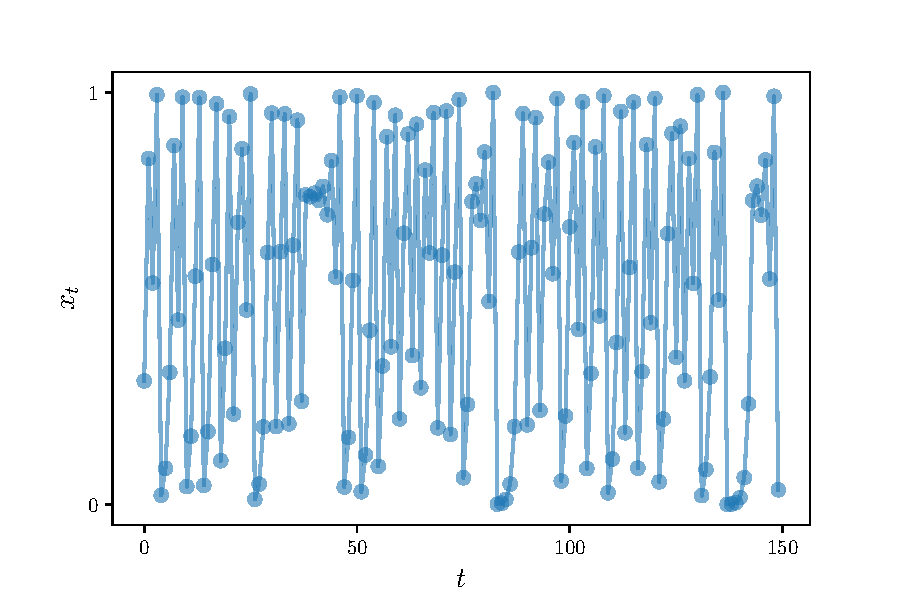
\includegraphics{chaos_intro_traj.pdf}}
    \end{figure}


\end{frame}


\begin{frame}
    
    
    \Eg Histogram

    \begin{figure}
        \centering
        \scalebox{.5}{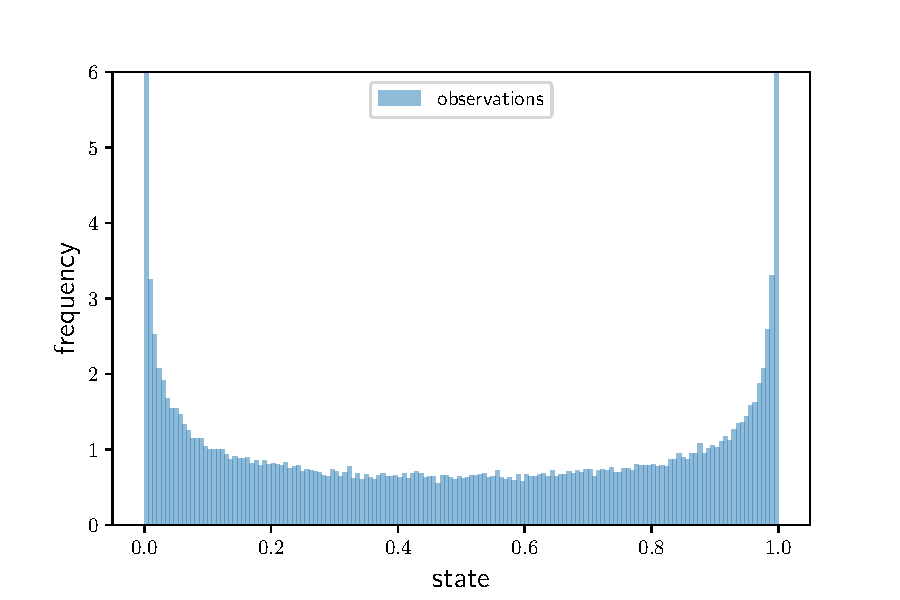
\includegraphics{chaos_intro_time_series_hist.pdf}}
    \end{figure}


\end{frame}

\begin{frame}
    
    
    \Eg Histogram

    \begin{figure}
        \centering
        \scalebox{.5}{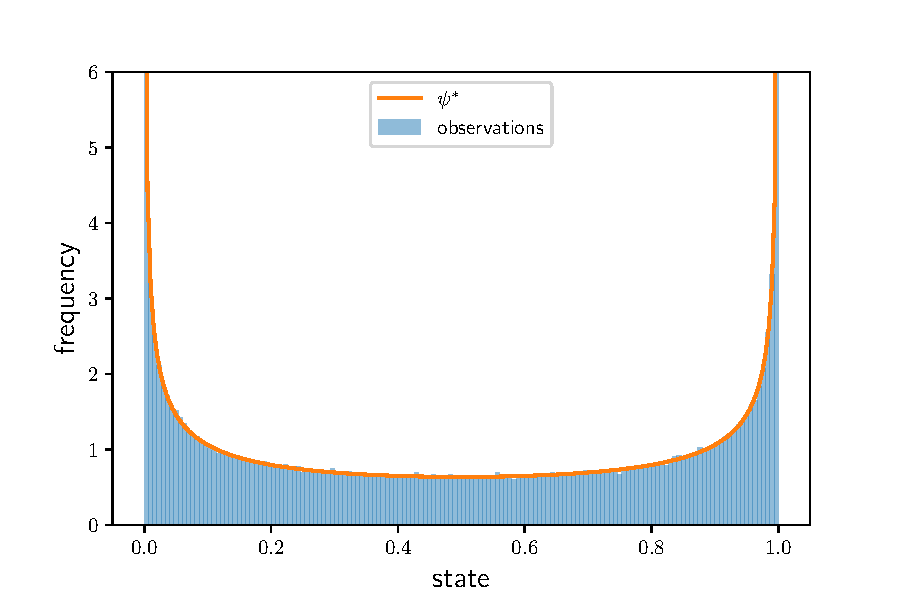
\includegraphics{chaos_intro_time_series_hist_fstar.pdf}}
    \end{figure}


\end{frame}


\begin{frame}
    \frametitle{Q3}
    
    In computational fluid dynamics, emerging research is exploring the
    replacement of robust computations with surrogate AI solvers. 

            \vspace{0.3em}
            \vspace{0.3em}
            \vspace{0.3em}
            \vspace{0.3em}
            \vspace{0.3em}
    Can we anticipate that AI might provide answers to complex economic
    problems if we forego understanding the mechanisms of economic phenomena?

\end{frame}

\begin{frame}
    
    Yes, and this can be valuable!

            \vspace{0.3em}
    \Eg \brown{Chinco, Clark-Joseph, Ye, Journal of Finance, 2020}

    \begin{itemize}
        \item Rolling 1 minute ahead return forecasts using lagged
            cross-section of returns
            \vspace{0.3em}
        \item Machine learning methods based on sparsity / shrinkage
            \vspace{0.3em}
        \item Significantly improved out-of-sample fit
    \end{itemize}

            \vspace{0.3em}
            \vspace{0.3em}
            \vspace{0.3em}
    The model is too complex for simple interpretations

            \vspace{0.3em}
            \vspace{0.3em}
    But it suggests that good predictors are correlated with news about
    fundamentals

\end{frame}

\end{document}


